\chapter{The Zeta Function of Riemann (Contd).}\label{chap13}

\setcounter{section}{7}
\section[The zeros of $\zeta(s)$]{The zeros of {\boldmath$\zeta(s)$}}\label{chap13:sec8}\pageoriginale

In the \ref{chap11}th Lecture, (p.98) we defined 
$$
\xi (s) \equiv \frac{1}{2} s (s-1) \pi^{-s/2}\Gamma (s/2) \zeta (s)
\equiv \frac{1}{2} s (s-1) \eta (s). 
$$
The following theorem about $\xi(s)$ is a consequence of the results
which we have already proved.

\setcounter{thm}{0}
\begin{thm}\cite[p.45]{key11}\label{chap13:thm1}
\begin{itemize}
\item[(i)] $\xi (s)$ is an entire function, and \
$\xi(s) = \xi (1-s)$;

\item[(ii)] $\xi (s)$ is real on $t=0$ and $\sigma =\frac{1}{2}$;

\item[(iii)] $\xi (0) = \xi (1) = \frac{1}{2}$.
\end{itemize}
\end{thm}

\begin{proof}
That $\xi (s) = \xi (1-s)$ is immediate from the functional equation
of $\zeta(s)$ (cf. p.97, Lecture \ref{chap11}). Clearly $\xi(s)$ is regular for
$\sigma >0$, and since $\xi (s) = \xi (1-s)$ it is also regular for
$\sigma < 1$, and hence it is entire.

This proves (i). 

$\xi (s)$ is obviously real for real $s$. Hence by a general theorem
it takes conjugate values at conjugate points. Thus $\xi \left(\frac{1}{2}
+ t i\right)$ and $\xi \left(\frac{1}{2} - ti\right)$ are conjugate; they are equal by
the functional equation. So they are real. This proves (ii).

To prove (iii) we observe that
$$
\xi (s) = \pi^{-s/2} \Gamma \left(\frac{s}{2}+1 \right) \cdot (s-1) \zeta(s),
$$
so that
$$
\xi (1) = \pi^{-1/2} \Gamma (3/2) \cdot 1 =\frac{1}{2},
$$
and by the functional equation, $\xi(0) =\frac{1}{2}$.
\end{proof}

We shall\pageoriginale next examine the location of the zeros of
$\xi(s)$ and of $\zeta(s)$.

\begin{thm}\cite[p.48]{key11}\label{chap13:thm2}
(i) The zeros of $\xi (s)$ (if any !) are all situated in the strip $0
\leq \sigma \leq 1$, and lie symmetrical about the lines $t=0$ and
$\sigma =\frac{1}{2}$

(ii) The zeros of $\zeta(s)$ are identical (in position and order of
multiplicity) with those of $\xi(s)$, except that $\zeta(s)$ has a
simple zero at each of the points $s=-2, -4. -6, \ldots$

(iii) $\xi(s)$ has no zeros on the real axis.
\end{thm}

\begin{proof}
(i) $\xi (s) = (s-1) \pi^{-s/2} \Gamma \left(\frac{s}{2}+1 \right)
  \zeta(s)$
$$
\equiv h(s) \zeta(s), \text{ say.}
$$

Now $\zeta(s) \neq 0$; for $\sigma >1$; (Euler Product!) also
$h(s) \neq 0$, for  $\sigma >1$;
hence $\xi (s) \neq 0$, for $\sigma > 1$;
hence $\xi (s) \neq 0$, for $\sigma < 0$; 
since $\xi(s) = \xi (1-s)$.

\begin{figure}[H]
\centering
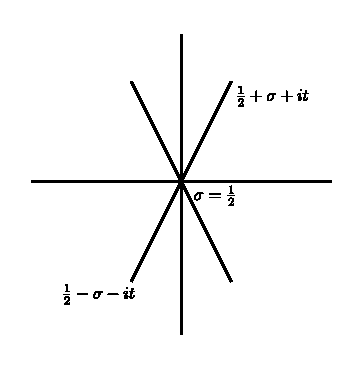
\includegraphics{figures/fig13.1.eps}
\end{figure}

The zeros, if any, are symmetrical about the real axis since $\xi
(\sigma \pm t i)$ are conjugates, and about \textit{the point} $s =
\frac{1}{2}$, since $\xi (s) = \xi (1-s)$; they are therefore also
symmetrical about the line $\sigma = \frac{1}{2}$.

(ii) The zeros of $\zeta(s)$ differ from those of $\xi (s)$ only in so
far as $h(s)$ has zeros or poles. The only zero of $h(s)$ is at
$s=1$. But this is not a zero of $\xi (s)$ since $\xi(1)=\frac{1}{2}$,
nor of $\zeta(s)$ for it is a pole of the latter.

The poles of $h(s)$ are simple ones at $s=-2, -4, -6, \ldots$. Since
these are points at which $\xi (s)$  is regular \textit{and not zero},
they must\pageoriginale be \textit{simple zeros} of $\zeta(s)$. We
have already seen this by a different argument on $p.95$.

(iii) Since $\xi(s)\neq 0$ for $\sigma <0$ and $\sigma >1$, it is
enough, in view of (ii), to show that
$$
\zeta(\sigma) \neq 0, \text{ for } 0 < \sigma <1.
$$
Now 
$$
(1-2^{1-s}) \zeta(s) = (1-2^{-s}) + (3^{-s} - 4^{-s}) + \cdots ,
\text{ for } \sigma > 0.
$$

To prove this we first notice that the relation is obvious for $\sigma
>1$, and secondly each side is regular for $\sigma >0$; the left side
is obviously regular for $\sigma >0$ (in fact it is entire); and, as
for the right side, we have
\begin{align*}
\left| \frac{1}{(2n-1)^s} - \frac{1}{(2n)^s} \right| & = \left|s
\int\limits^{2n}_{2n-1} \frac{dx}{x^{s+1}} \right|\\
& \leq \frac{|s|}{(2n-1)^{\sigma +1}} < \frac{\Delta}{(2n-1)^{\delta+1}}
\end{align*}
if $\sigma > \delta$ and $|s| < \Delta$ for any fixed $\delta$ and
$\Delta$ 

But, if $0 < \sigma < 1 $, the above relation gives
$$
(1-2^{1-\sigma}) \zeta(\sigma) >0, \text{ or } \zeta(\sigma) <0.
$$
This establishes (iii).
\end{proof}

\begin{remarks*}
The strip $0 \leq \sigma \leq 1$ is called the `\textit{critical
  strip}'; the line $\sigma = \frac{1}{2}$ the `critical line'; the
zeros at $-2, -4, -6, \ldots$ are the `\textit{trivial zeros}' of
$\zeta(s)$. We still have to show that $\xi(s)$ actually has zeros,
i.e. $\zeta(s)$ has `non-trivial'\pageoriginale zeros. This is done by
an appeal to the theory of entire functions gives in the first few
lectures.
\end{remarks*}

\begin{thm}\cite[p.56]{key11}\label{chap13:thm3}
If $M(r) \equiv \max\limits_{|s| =r} |\xi(s)|$, then 
$$
\log M(r) \sim \frac{1}{2} r \log r, \text{ as } r \to \infty
$$
\end{thm}

\begin{proof}
For $\sigma \geq 2$, we have
$$
|\zeta(s)| \leq \zeta(2),
$$
and for $\sigma \geq \frac{1}{2}$, $|t| \geq 1$, we have
$$
|\zeta(s)| < c_1 |t|^{1/2},
$$
so that
$$
|\zeta(s)| < c_2 |s|^{1/2}, \text{ for } \sigma \geq \frac{1}{2}, |s|>3.
$$
Applying Stirling's formula to $\Gamma (s/2)$, we get, for 
\begin{align*}
\sigma \geq \frac{1}{2}, \; \; |s| & = r >3,\\
|\xi (s)| & < e^{|\frac{1}{2} s \log \frac{1}{2}s| + c_3 |s|} \\
& < e^{\frac{1}{2}r \log r + c_4 r},
\end{align*}
since $\log \dfrac{s}{2} = \log|s| - \log 2+i\arg s $, $|\arg s|<
\frac{\pi}{2}$. 
From the equation $\xi(s) = \xi (1-s)$, we infer that
\begin{align*}
|\xi (s)| & < e^{\frac{1}{2} |1-s| \log |1-s| + c_4 |1-s|}\\
& < e^{\frac{1}{2} r \log r+ c_5 r}
\end{align*}
for $\sigma \leq \frac{1}{2}$, $|s| = r >4$. Combining the results we
get
$$
M(r) < e^{\frac{1}{2} r \log r + c_6 r}, r >4.
$$

On the\pageoriginale other hand, if $r>2$,
$$
M(r) \geq \xi (r) > 1. \pi^{-\frac{1}{2} r} \Gamma \left(\frac{1}{2}r \right)
e^{\frac{1}{2} r \log r - c_7 r} 
$$
Thus we have, for $r>4$,
$$
\frac{1}{2} r \log r -C_7 r < \log M(r) < \frac{1}{2} r \log r + c_6 r,
$$
and hence the result.
\end{proof}

\begin{thm}\cite[p.57]{key11}\label{chap13:thm4} 
\begin{itemize}
\item[(i)] $\xi(s)$ has an infinity of zeros;

\item[(ii)] If they are denoted by `$\rho$', then $\sum
  |\rho|^{-\alpha}$ converges for $\alpha>1$, diverges for $\alpha
  \leq 1$;

\item[(iii)] 
$
\xi (s) = e^{b_0 + b_1 s} \pi_{\rho} \left\{ \left(1-\frac{s}{\rho} \right) 
e^{s/\rho}\right\} ,
$ \ where $b_0$, $b_1$ are constants;

\item[(iv)] $\dfrac{\xi'(s)}{\xi(s)} = b_1 + \sum
  \left(\dfrac{1}{s-\rho} + \dfrac{1}{\rho}\right)$ 

\item[(v)] $\dfrac{\zeta'(s)}{\zeta(s)} = b - \dfrac{1}{s-1} -
  \frac{1}{2} \dfrac{\Gamma'}{\Gamma} \left(\dfrac{s}{2}+1 \right)+
  \sum\limits_\rho \left(\dfrac{1}{s-\rho} + \dfrac{1}{\rho} \right)$,   
\end{itemize}
where  $b=b_1 + \frac{1}{2} \log 2 \pi$.
\end{thm}

\begin{proof}
$\xi (0) = \frac{1}{2} \neq 0$, and we apply the theory of entire
  functions as developed in the earlier lectures. By Theorem \ref{chap13:thm3}, $\xi
  (s)$ is of order 1, and the relation $\log M(r) = O(r)$ does not
  hold. Hence $\rho_1 =1$, $\xi(s)$ has an infinity of zeros and $\sum
  \frac{1}{|\rho|}$ diverges (by a previous theorem). This proves
  (i), (ii) and (iii). (iv) follows by logarithmic
  differentiation. (v) is obtained from $\xi (s) = (s-1) \pi^{-s/2}
  \Gamma (\frac{s}{2}+1) \zeta(s)$.
 

We shall now show that $\zeta(s)$ has no zeros on the line $\sigma
=1$. 
\end{proof}

\begin{thm}\cite[p.28]{key11}\label{chap13:thm5}
$\zeta (1+i t) \neq 0$.
\end{thm}

\medskip
\noindent{\textbf{First Proof.}}
$2(1+\cos \theta t)^2 = 3 + 4 \cos \theta + \cos 2 \theta \geq
0$\pageoriginale for real $\theta$. Since
$$
\log \zeta(s) = \sum\limits_m \sum\limits_p \frac{1}{mp^{ms}}, \text{
  for } \sigma >1,
$$
we have
\begin{align*}
\log |\zeta(s)| & = \re \sum\limits^\infty_{n=2} c_n n^{-\sigma - t
  i}\\
& = \sum\limits^\infty_{n=2} c_n n^{-\sigma } \cos (t \log n),
\end{align*}
where $c_n = \begin{cases}
1/m & \text{ if $n$ is the $m^{\rm th}$ power of a prime}\\
0 & \text{ otherwise}.
\end{cases}
$

Hence
\begin{align*}
\log & \left| \zeta^3 (\sigma) \cdot \zeta (\sigma + ti) \zeta (\sigma
+ 2 ti)\right|\\
& = \sum c_n n^{-\sigma} \left\{3+4 \cos (t \log n) + \cos (2t \log n)
\right\} \\
& \geq 0,
\end{align*}
because $c_n \geq 0$ and we have the trigonometric identity above.

Thus 
$$
\left\{(\sigma -1) \zeta (\sigma) \right\}^3 \left|\frac{\zeta(\sigma
  + ti)}{\sigma -1} \right|^4 |\zeta (\sigma + 2 ti)| \geq
\frac{1}{\sigma -1},
$$
if $\sigma >1$.

Now suppose $1+ti(t \gtrless 0)$ were a zero of $\zeta(s)$; then, on
letting $\sigma \to 1+0 $, we see that the left hand side in the above
inequality would tend to a finite limit, viz. $|\zeta'(1+ti)|^4
|\zeta(1+2ti)|$, while the right\pageoriginale hand side tends to
$\infty$. Hence $\zeta(1+it) \neq 0$.

\medskip
\noindent{\textbf{Second Proof.}}
\cite[p.89]{key11} 
We know from the \ref{chap8}th Lecture (1.12) that if $\alpha$ is real, and
$\alpha \neq 0$, then 
\begin{equation*}
f(s) \equiv \frac{\zeta^2 (s) \zeta(s-\alpha i) \zeta(s+\alpha
  i)}{\zeta(2s)} = \sum\limits^\infty_{n=1} \frac{|\sigma_{\alpha
    i}(n)|^2}{n^s}, \sigma >1 \tag{8.1}\label{c13:eq8.1}
\end{equation*}
Let $\sigma_0$ be the abscissa of convergence of the series on the
right hand side. Then $\sigma_0 \leq 1$. The sum-function of the
series is then regular in the half-plane $\sigma > \sigma_0$, and
hence, by analytic continuation, (\ref{c13:eq8.1}) can be upheld for $\sigma >
\sigma_0$. And since the coefficients of the series are positive, the
point $s =\sigma_0$ is a singularity of $f(s)$.

Now, if $1+\alpha i$ is a zero of $\zeta(s)$, then so is $(1-\alpha
i)$, and these two zeros cancel the double pole of $\xi^2 (s)$ at
$s=1$. Hence $f(s)$ is regular on the real axis, as far to the left as
$s=-1$, where $\zeta(2s) =0$. Hence $\sigma_0=-1$. This is, however,
impossible since (\ref{c13:eq8.1}) gives
$$
f \left(\frac{1}{2} \right) \geq \left| \sigma_{\alpha i} (1)\right|^2 = 1,
$$
while $f(\frac{1}{2}) =0$. Thus $\zeta(1+\alpha i) \neq 0$.

\begin{remarks*}
\begin{itemize}
\item[(i)] We shall show later on that this fact $(\zeta (1+it) \neq
  0)$ is equivalent to the Prime Number Theorem. 

\item[(ii)] If $\rho = \beta + \gamma i$ is a zero of $\xi (s)$, then
  we have seen that $0 \leq \beta \leq 1$, and since $\zeta (1+it)
  \neq 0$, we actually have $0 \leq \beta <1$, and by symmetry about
  the line $\sigma = \frac{1}{2}$, we have $0< \beta < 1$. 
\end{itemize}
\end{remarks*}
